\documentclass[../../thesis.tex]{subfiles}

\newcommand{\inner}[2]{\left<#1, #2\right>}
\newcommand{\alemap}{\ensuremath{\mathcal{A}}}
\newcommand{\dt}{\ensuremath{\Delta t}}
\newcommand{\pexp}{\ensuremath{\frac{2\gamma}{\left(\gamma-1\right)}}}
\newcommand{\aleX}{\ensuremath{\mathcal{X}}}
\newcommand{\Ah}[1]{\ensuremath{\vb{#1}^{n+1}_h}}
\newcommand{\Ahn}[1]{\ensuremath{\vb{#1}^{n}_h}}

\newcommand{\rbV}{\ensuremath{\mathbb{V}}}
\newcommand{\rbVT}{\ensuremath{\rbV^T}}
\newcommand{\epspod}{\ensuremath{\varepsilon_\text{POD}}}

\begin{document}

% \section{Arbitrary Mesh Displacement}
% We introduce an arbitrary distortion to the mesh,
% to mimick the effects of mesh adapting techniques.
% We take a generic density function with a Gaussian bell as a proxy,
% \begin{equation}
%     \mathcal{F}\qty(\aleX) &= p \cdot \exp(-\qty(\frac{\aleX - x_c}{\sigma_c})^2),
% \end{equation}
% where three geometrical parameters are defined:
% \begin{itemize}
%     \item $x_c$: location;
%     \item $\sigma_c$: span,
%     \item $y_0$: magnitude.
% \end{itemize}
% This will concentrate nodes on a specific region of the domain.
% Then, for $\aleX \in \Omega_0$, where $\Omega_0 = \qty[0, L_0]$ is the fixed reference domain,
% we have the following transformation in terms of a mesh displacement,
% \begin{subequations}
%     \begin{align}
%         x &= \aleX + d\qty(\aleX, t),
%         \label{eq:displacement_definition}
%         \\[2mm]
%         d\qty(\aleX, t) &= \aleX \cdot \qty[1 + \mathcal{F}\qty(\aleX)] \qty(\hat{L}(t) - 1),
%         \\[2mm]
%         \hat{L}(t) &= 1 - \delta \cdot \qty(1 - \cos(\omega t)).
%         % \\[5mm]
%         % d\qty(\aleX, t) &= \qty[\aleX + \aleX \cdot \mathcal{F}\qty(\aleX)] \qty(\hat{L}(t) - 1)
%         % \\[2mm]
%         % d\qty(\aleX, t) &= 
%         %   \aleX \cdot \qty(\hat{L}(t) - 1) 
%         % + \aleX \cdot \qty(\hat{L}(t) - 1) \cdot \mathcal{F}\qty(\aleX)
%         % \\[5mm]
%         % d\qty(\aleX, t) &= \aleX \qty[1 + y_0 \cdot \exp(-\qty(\frac{\aleX - x_c}{\sigma_c})^2)] \qty(\hat{L}(t) - 1)
%     \end{align}
% \end{subequations}
% This displacement contains the piston oscillation 
% and the arbitrary concentration of mesh nodes.

% \subsection{Effects on the Mesh Size}
% We demonstrate the effects of the arbitrary displacement in the mesh step size.
% Evaluating Equation~(\ref{eq:displacement_definition}) at two consecutive nodes
% and computing their difference,
% \begin{subequations}    
% \begin{align}
%     \Delta x_i &= x_i - x_{i-1},
%     \\[2mm]
%     \Delta x_i &= \aleX_i - \aleX_{i-1} + \qty(d\qty(\aleX_i, t) - d\qty(\aleX_{i-1}, t)),
%     \\[2mm]
%     \Delta x_i &= \Delta \aleX_i + \qty(d\qty(\aleX_i, t) - d\qty(\aleX_{i-1}, t)),
%     \\[2mm]
%     \Delta x_i &= 
%     \underbrace{\Delta \aleX_i \cdot \hat{L}(t)}_{\text{Uniform stretching}}
%     \nonumber\\
%     &+\qty[\aleX_i \cdot \mathcal{F}\qty(\aleX_i)
%     - \aleX_{i-1} \cdot \mathcal{F}\qty(\aleX_{i-1})] \cdot \qty(\hat{L}(t) - 1);
%     \end{align}
% \end{subequations}
% we arrive to an expression for the mesh size $\Delta x_i$ 
% as a function of the reference mesh size and position.
% If the function $\mathcal{F}$ was set to zero, 
% we would recover a uniform stretching of the reference domain.
% % \begin{align}
% %     \begin{split}
% %         d\qty(\aleX_i, t) - d\qty(\aleX_{i-1}, t) 
% %         &= \qty[\aleX_i - \aleX_{i-1}] \cdot \qty(\hat{L}(t) - 1)
% %         \\
% %         + 
% %         &\qty[\aleX_i \cdot \mathcal{F}\qty(\aleX_i)
% %         - \aleX_{i-1} \cdot \mathcal{F}\qty(\aleX_{i-1})] \cdot \qty(\hat{L}(t) - 1) 
% %     \end{split}
% %     \\[2mm]
% %     \begin{split}
% %         d\qty(\aleX_i, t) - d\qty(\aleX_{i-1}, t) 
% %         &= \Delta \aleX_i \cdot \qty(\hat{L}(t) - 1)
% %         \\
% %         + 
% %         &\qty[\aleX_i \cdot \mathcal{F}\qty(\aleX_i)
% %         - \aleX_{i-1} \cdot \mathcal{F}\qty(\aleX_{i-1})] \cdot \qty(\hat{L}(t) - 1) 
% %     \end{split}
% % \end{align}

% \subsubsection{Mesh Quality}
% Not all geometrical parametrizations of the mesh displacement are valid.
% As shown in Table~\ref{tab:mesh_disp_params}, some parametrizations
% lead to non-invertible mappings.
% This takes place when the displacement is so large locally 
% that the mesh nodes ordering is lost in the physical domain.
% When this happens, two points in the reference domain map to the same point in the physical space.
% \begin{table}[h]
%     \centering
%     \caption{Mesh deformation parametrizations.}
%     \begin{tabular}{lccccc}
%         \toprule
%         {}                                      & $\delta$ & $x_c$                & $\sigma_c$           & $y_0$  & Invertible \\
%         \midrule
%         Figure~\ref{fig:mesh_disp_compression}  & \multirow{3}{*}{0.3}         & \multirow{3}{*}{0.5} & \multirow{3}{*}{0.1} & 0.5    & \multirow{2}{*}{Yes} \\
%         Figure~\ref{fig:mesh_disp_expansion}    &          &           &                      & 0.75   & \\ 
%         % \midrule[0.01mm]
%         Figure~\ref{fig:mesh_disp_expansion_unfeasible} &  &           &                      & 1.75   & No \\
%         \bottomrule
%     \end{tabular}        
%     \label{tab:mesh_disp_params}
% \end{table}

% The correct procedure to deal with the mesh feasibility problem 
% would be to compute the Jacobian analytically
% and derive from it upper and lower bounds for each parameter.
% However, for such a simple domain transformation, 
% we opt to check numerically at runtime if the mesh is feasible or not.
% In fact, to prevent round-off errors,
% we impose a lower bound on the mesh step size. 
% When it is breached,
% \begin{equation}
%     \forall \, i \quad &\Delta x_i < 10^{-6}, 
% \end{equation}
% we discard that parametrization.

% \begin{figure}[h]
%     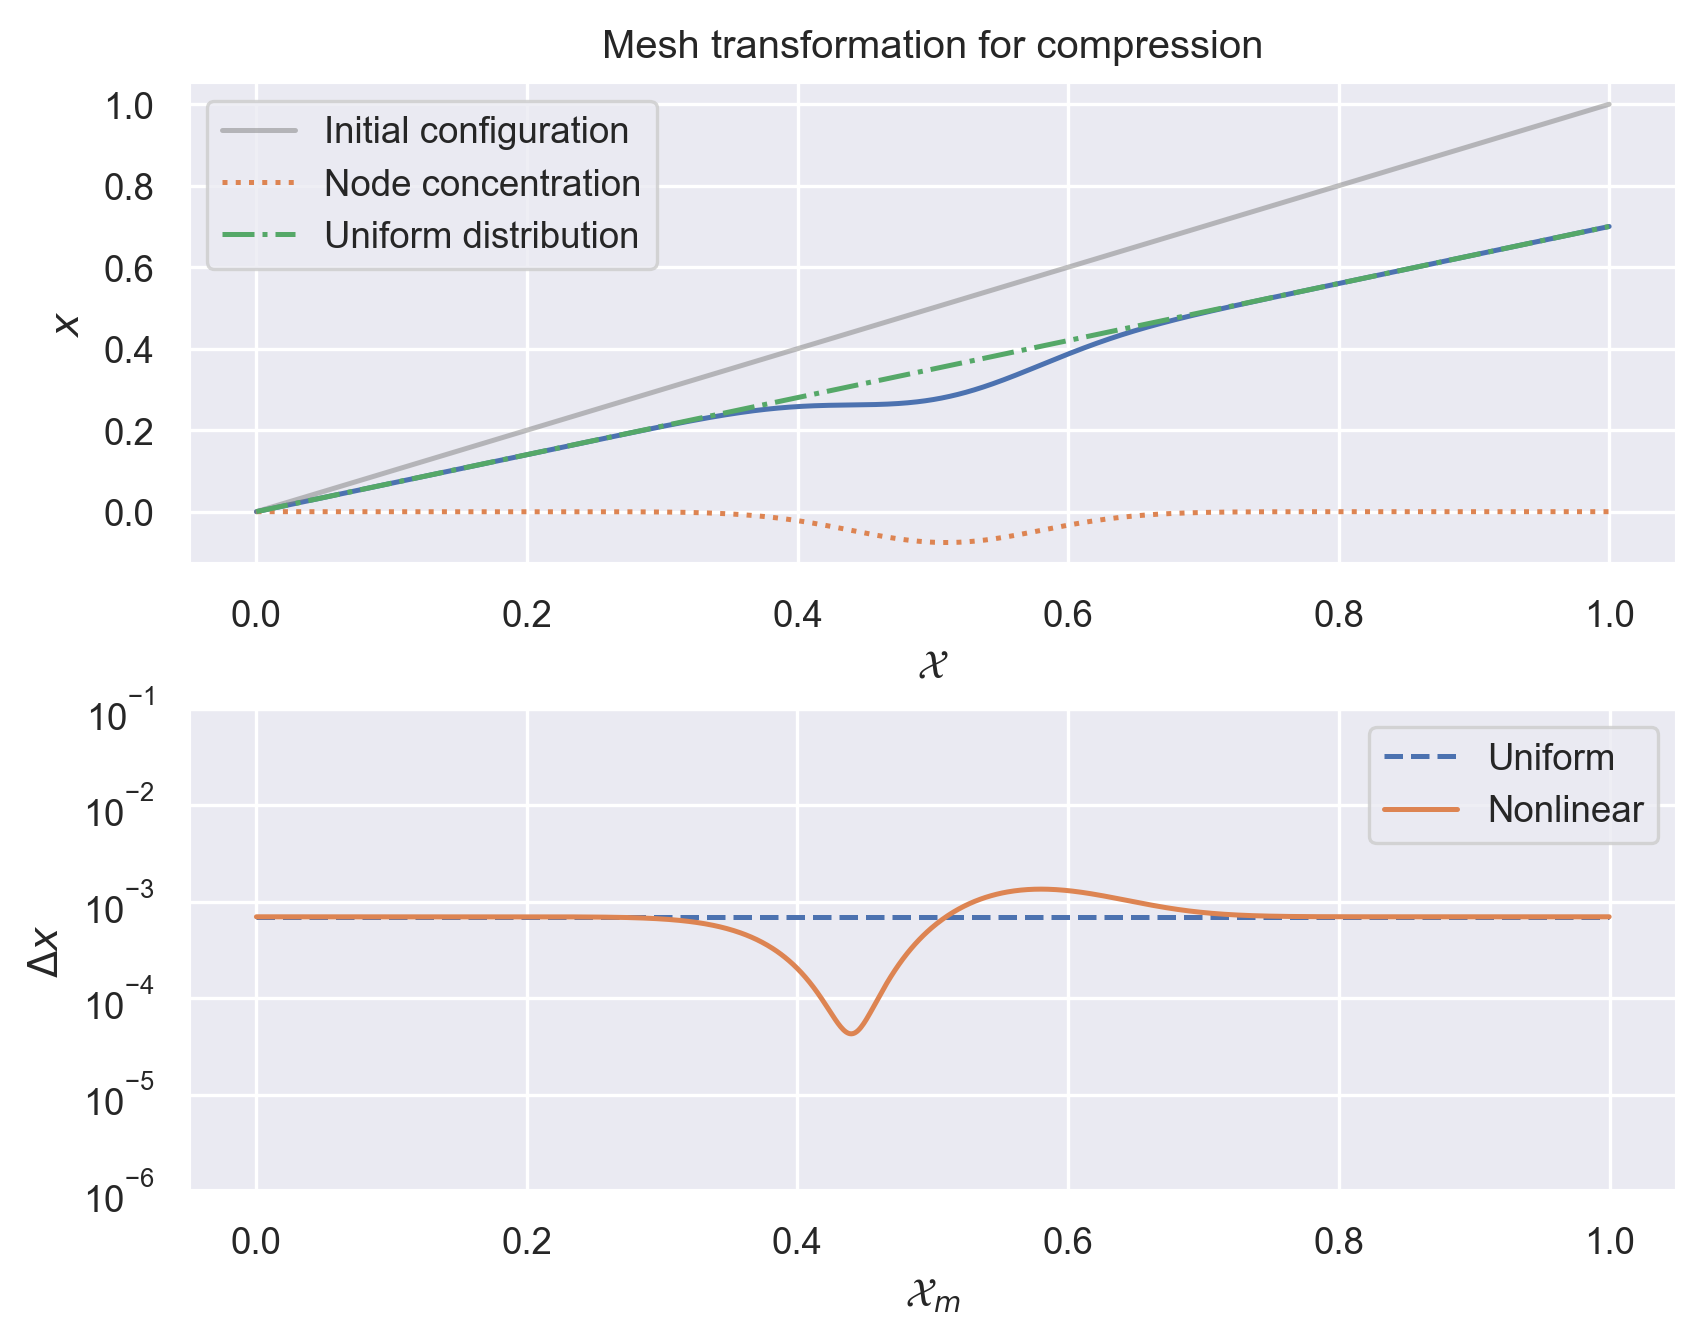
\includegraphics[width =\columnwidth]{research_project/piston/figures/nonlinear_displacement/separable/mapping_mu_05_sigma_01_p_05_compression.png}
%     \caption{Feasible mesh compression. 
%     The green line shows the maximum piston compression.
%     The nodes are locally compressed to the left of the Gaussian curve.}
%     \label{fig:mesh_disp_compression}
% \end{figure}
% \begin{figure}[h]
%     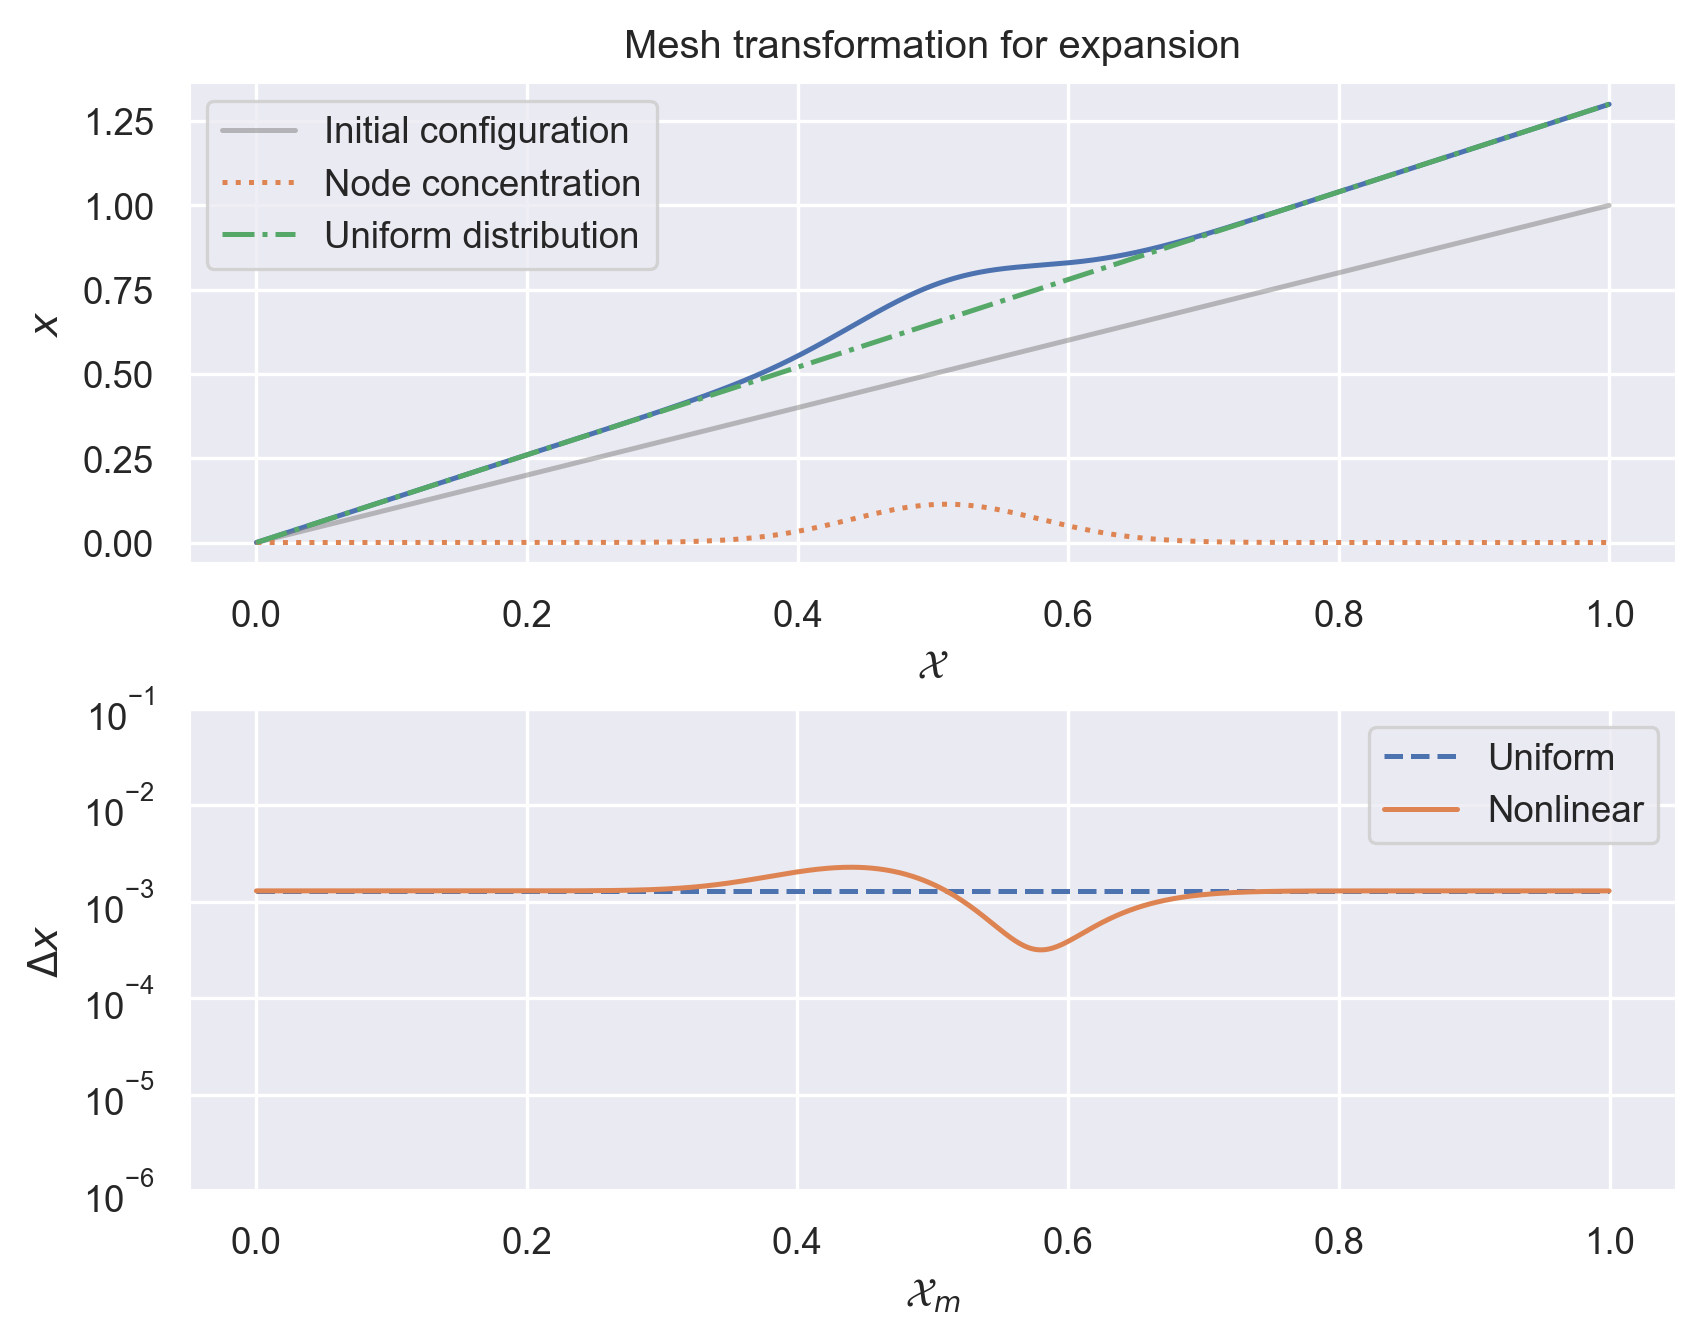
\includegraphics[width =\columnwidth]{research_project/piston/figures/nonlinear_displacement/separable/mapping_mu_05_sigma_01_p_075_expansion.png}
%     \caption{Feasible mesh expansion. 
%     The green line shows the maximum piston expansion.
%     The nodes are locally compressed to the right of the Gaussian curve.}
%     \label{fig:mesh_disp_expansion}
% \end{figure}
% \begin{figure}[h]
%     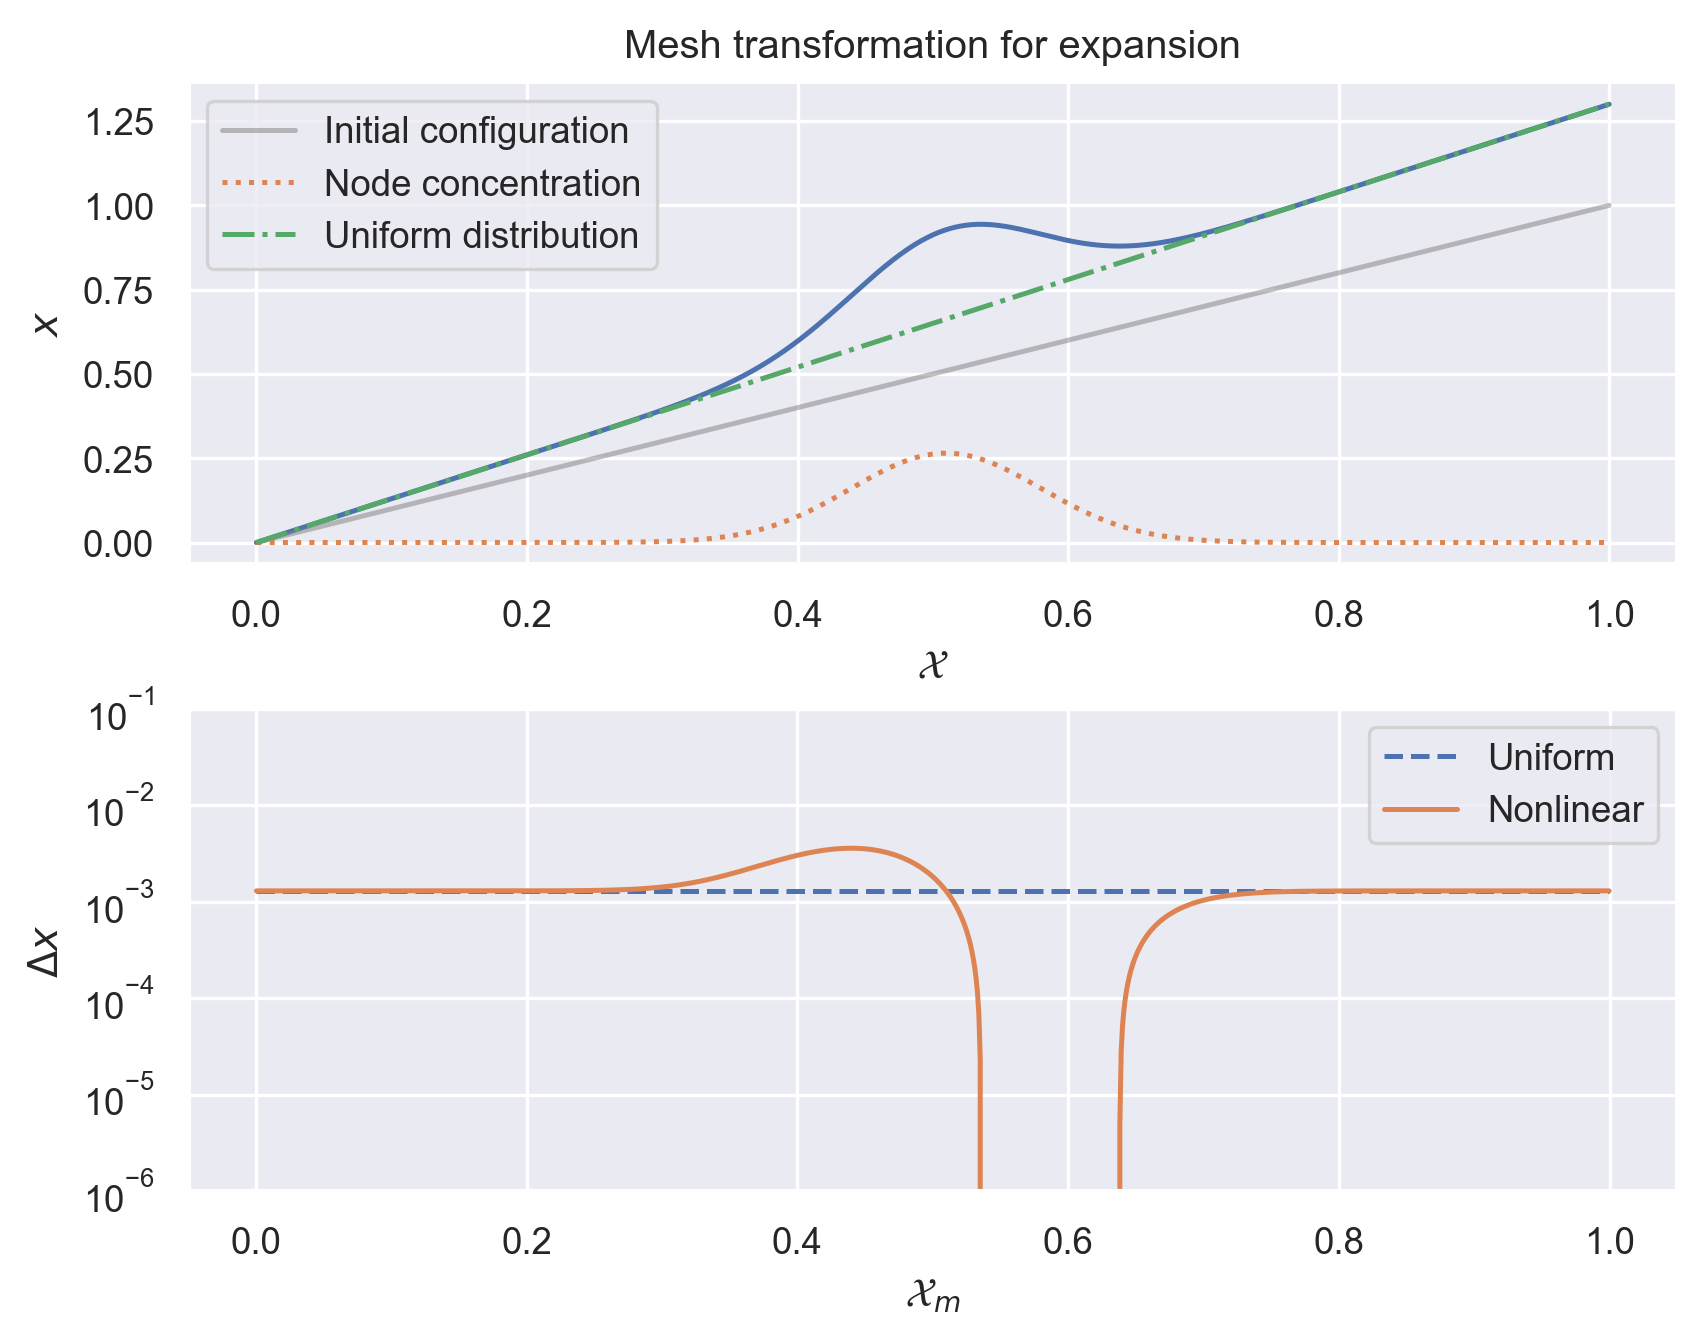
\includegraphics[width =\columnwidth]{research_project/piston/figures/nonlinear_displacement/separable/mapping_mu_05_sigma_01_p_175_expansion.png}
%     \caption{Unfeasible mesh expansion.
%     Due to the large mesh distortion, the ordering is lost in the physical domain,
%     leading to negative mesh step sizes.}
%     \label{fig:mesh_disp_expansion_unfeasible}
% \end{figure}

\subsection{Reduction Results}
We present the reduction achieved by the nested POD.
We recall that this algorithm is used for the solution and the snapshots of each operator.
The reduction methodology introduced by the (M)DEIM technique 
is the selection of the interpolation entries, 
which will guarantee a correct approximation of the operator when they are exactly matched.

In Table~\ref{tab:nlinear_disp_bases_size} we give the resulting basis size 
for each operator at each step of the nested POD.
The final size (\mbox{"Param. space"} column) is sufficient to accurately reconstruct the operators.
% As opposed to the initial scenario of uniform cell distortion, 
% where the Jacobian was only a function of time, we
All operators require more than a trivial number of elements, 
but the bases size differ.
The most difficult operator is the trilinear one.

The trilinear term snapshots have been obtained from the FOM simulation.
Since these snapshots contain simultaneously 
the effects of the solution 
and the nonlinear Jacobian,
the reduction of this operator requires as many terms as the solution space.

We have purposefully used a different parameter sampling size 
for the FOM simulation and the collection of operator snapshots;
to show a weakness of this methodology.
Assembling operators is a time-consuming operation, 
but it is cheaper than carrying out a full FEM simulation.
Hence, it is encouraged to have a methodology which splits the collection
of operator snapshots and solution snapshots.
The former are cheaper to obtain than the latter, 
and hence a larger parameter space can be sampled to produce a richer reduced basis.
By richer basis we intend one that is likely to work better during the online stage, 
for it has potentially a higher generalization degree.

A possible scenario where the split between the assembly and snapshot-collection steps
could not be feasible would be one where the displacement had to track the solution of the PDE.
In that case we have no alternative than to collect 
\textit{all} the snapshots (operators and solution) from FEM simulations;
knowing that the reduction will have to deal with both effects simultaneously. 

Within the operators which do not depend on the solution,
the most difficult one is the \textit{Stiffness} operator. 
We believe this is so because it contains two gradient operations,
on the test and trial functions respectively.
A gradient operation implies the existence of an inverse mesh size term \mbox{$h^{-1}(x,t)$}.
Since the mesh is no longer uniform, 
the interaction \mbox{$h_{i}^{-1} h_{j}^{-1}$} between the two gradients will produce a tougher nonlinearity
than the one produced by a single gradient or none, 
as shown by the reduction of the remaining operators.

\begin{table}[h]
    \centering
    \caption{Basis size at each step of the nested POD strategy.
    The operators are sorted by their collateral basis size.}
    \begin{tabular}{lccc}
        \toprule
        {} &  Time int. ($N_t = 500$) &  Param. space & $N_{\mu}$ \\
        \midrule
        Reduced-basis     &                     660 &          93 & 20 \\
        \midrule[0.01mm]
        Trilinear         &                     670 &          94 & 20 \\
        Stiffness         &                     121 &          68 & \multirow{5}{*}{30} \\
        Rhs               &                     180 &          32 &  \\
        Mass              &                      60 &          21 &  \\
        Convection        &                      60 &          20 &  \\
        Nonlinear-lifting &                      60 &          19 &  \\
        \bottomrule
    \end{tabular}        
    \label{tab:nlinear_disp_bases_size}
\end{table}

In Figure~\ref{fig:nlinear_disp_sep_loglog} we show 
the singular value decay (SV decay) for each operator.
% Top plot
On the top plot, we present the decays for each time integration path 
(for a fixed parameter, they represent the branches of the nested POD).
These decays correspond to the first compression of the snapshots, 
with which we obtain a basis $\Psi_{\mu_i}$ for a specific parametrization.
% Bottom plot
On the bottom plot, we present the decay of the final POD compression, 
which compresses (for each operator) all of the previous bases into one.

% Zoom-in
% We observe how the Stiffness and RHS operators are tougher to reduce in time,
% and hence also in the parameter space.
In Figure~\ref{fig:nlinear_disp_sep_logy} we present 
a zoom-in for the first ten singular values.
This shows how some operators are reduced 
to very few elements in the time direction.

% Discussion 
Indeed, in the time direction most operators still remain simple to reduce, 
but when each parameter-fixed basis is compressed with the others,
most information is retained.
This is so because the mesh parameters have a nonlinear effect, 
whereas time has a linear one.
That is why in time it is simple to reduce the operator,
but not so much across the geometrical parameter space.
When we were dealing with a uniform deformation of the mesh,
since the stretching parameter $\delta$ is present linearly,
the piston oscillation could be captured by sampling one parametrization,
two at most\footnote{The oscillating frequency $\omega$ is inside a sinusoidal function,
but this was only relevant for the mesh velocity, 
not the overall displacement.}.

\begin{figure}[h]
    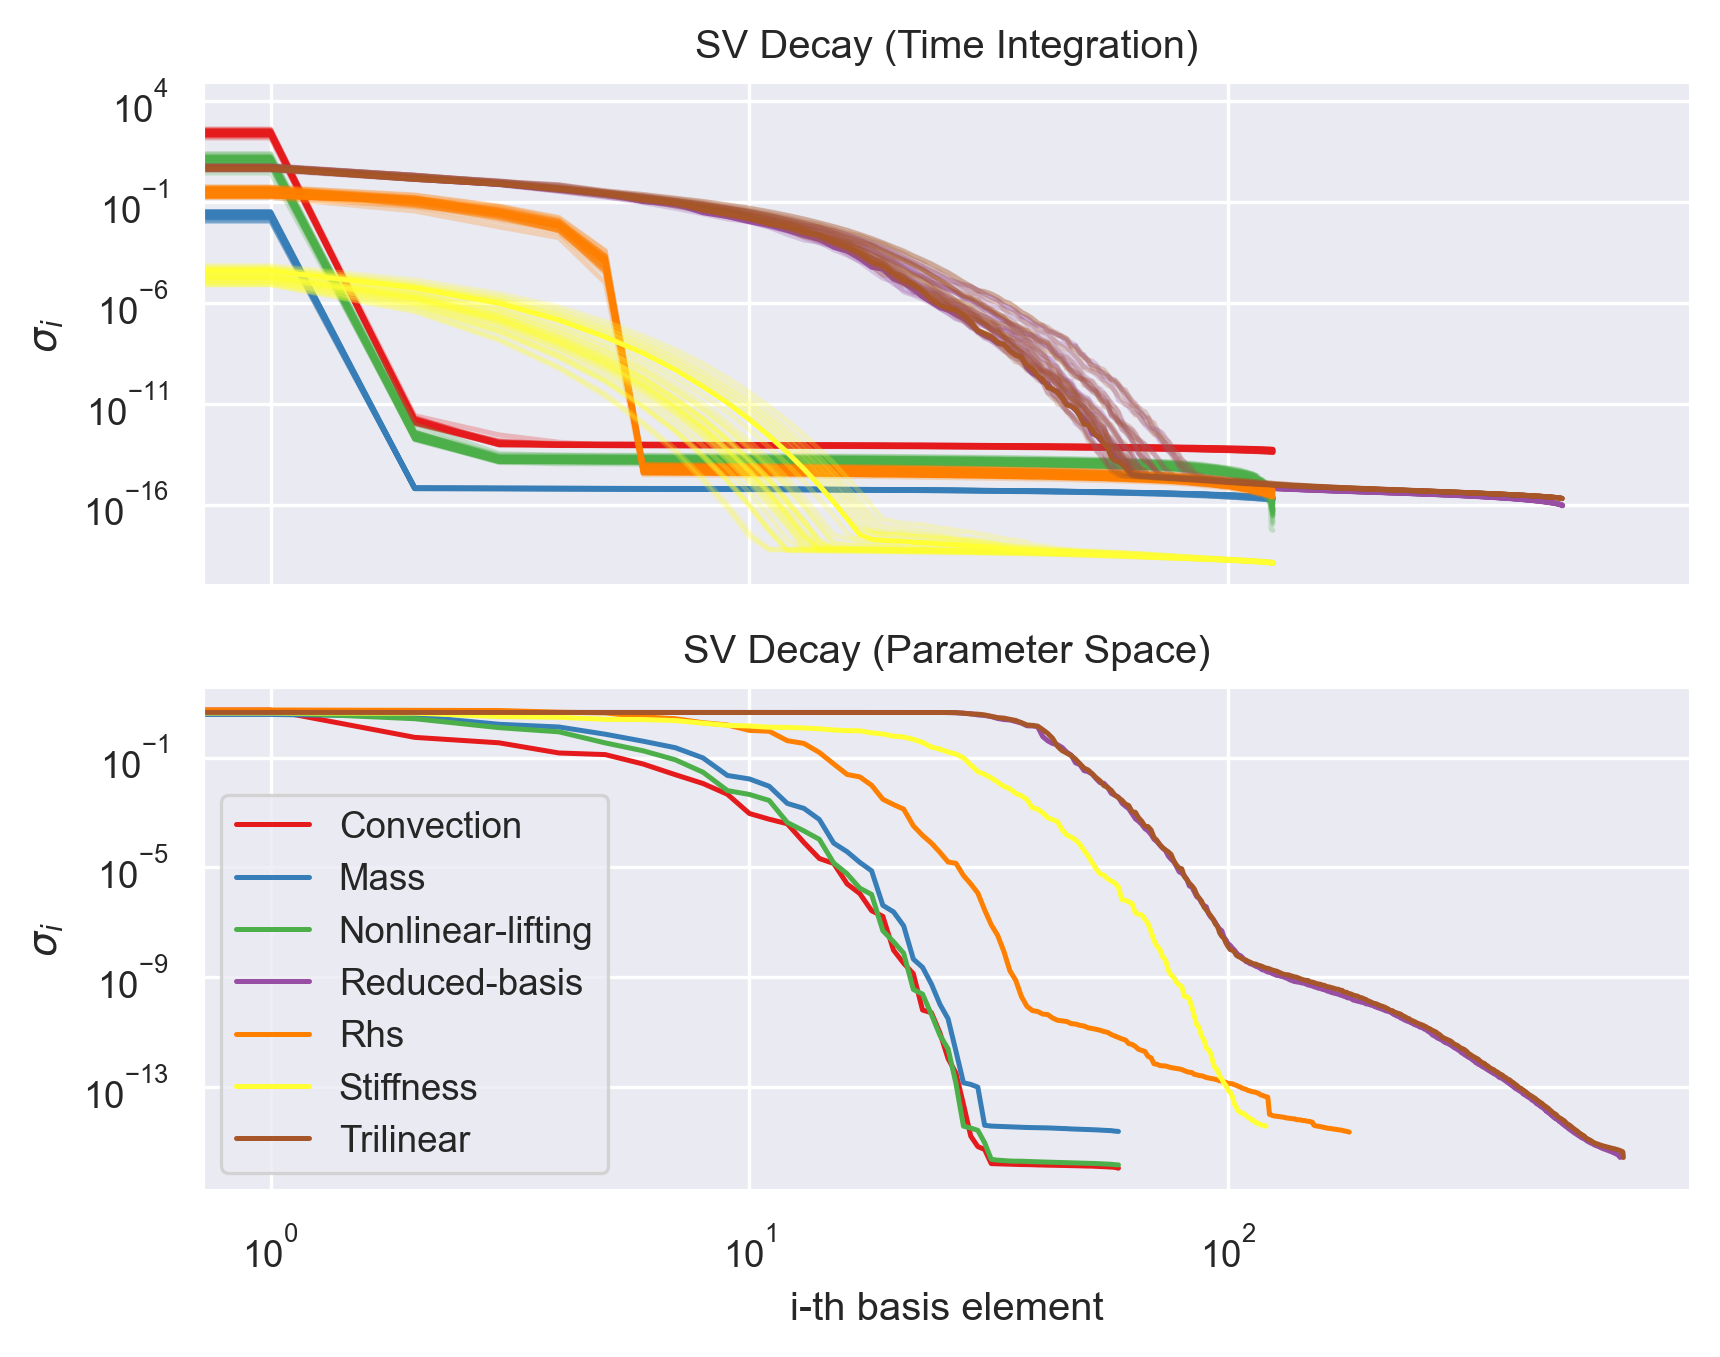
\includegraphics[width =\columnwidth]{research_project/piston/figures/nonlinear_displacement/separable/sigmas_loglog.png}
    \caption{Singular value decay for the two nested POD steps: 
    \mbox{time integration} (top) and \mbox{parameter space} (bottom).
    Both axes are represented in logarithmic scale.
    We observe how due to the presence of the nonlinear displacement
    the operators are no longer trivially reduced.
    It takes several basis terms to accurately represent 
    the effects of the nonlinearity.
    The solution space and the trilinear operator have an identical decay.
    This is so because the trilinear form is equally affected by the 
    values of the extrapolated velocity $u^{*}$ 
    and the effects of the nonlinear displacement.}
    \label{fig:nlinear_disp_sep_loglog}
\end{figure}

\begin{figure}[h]
    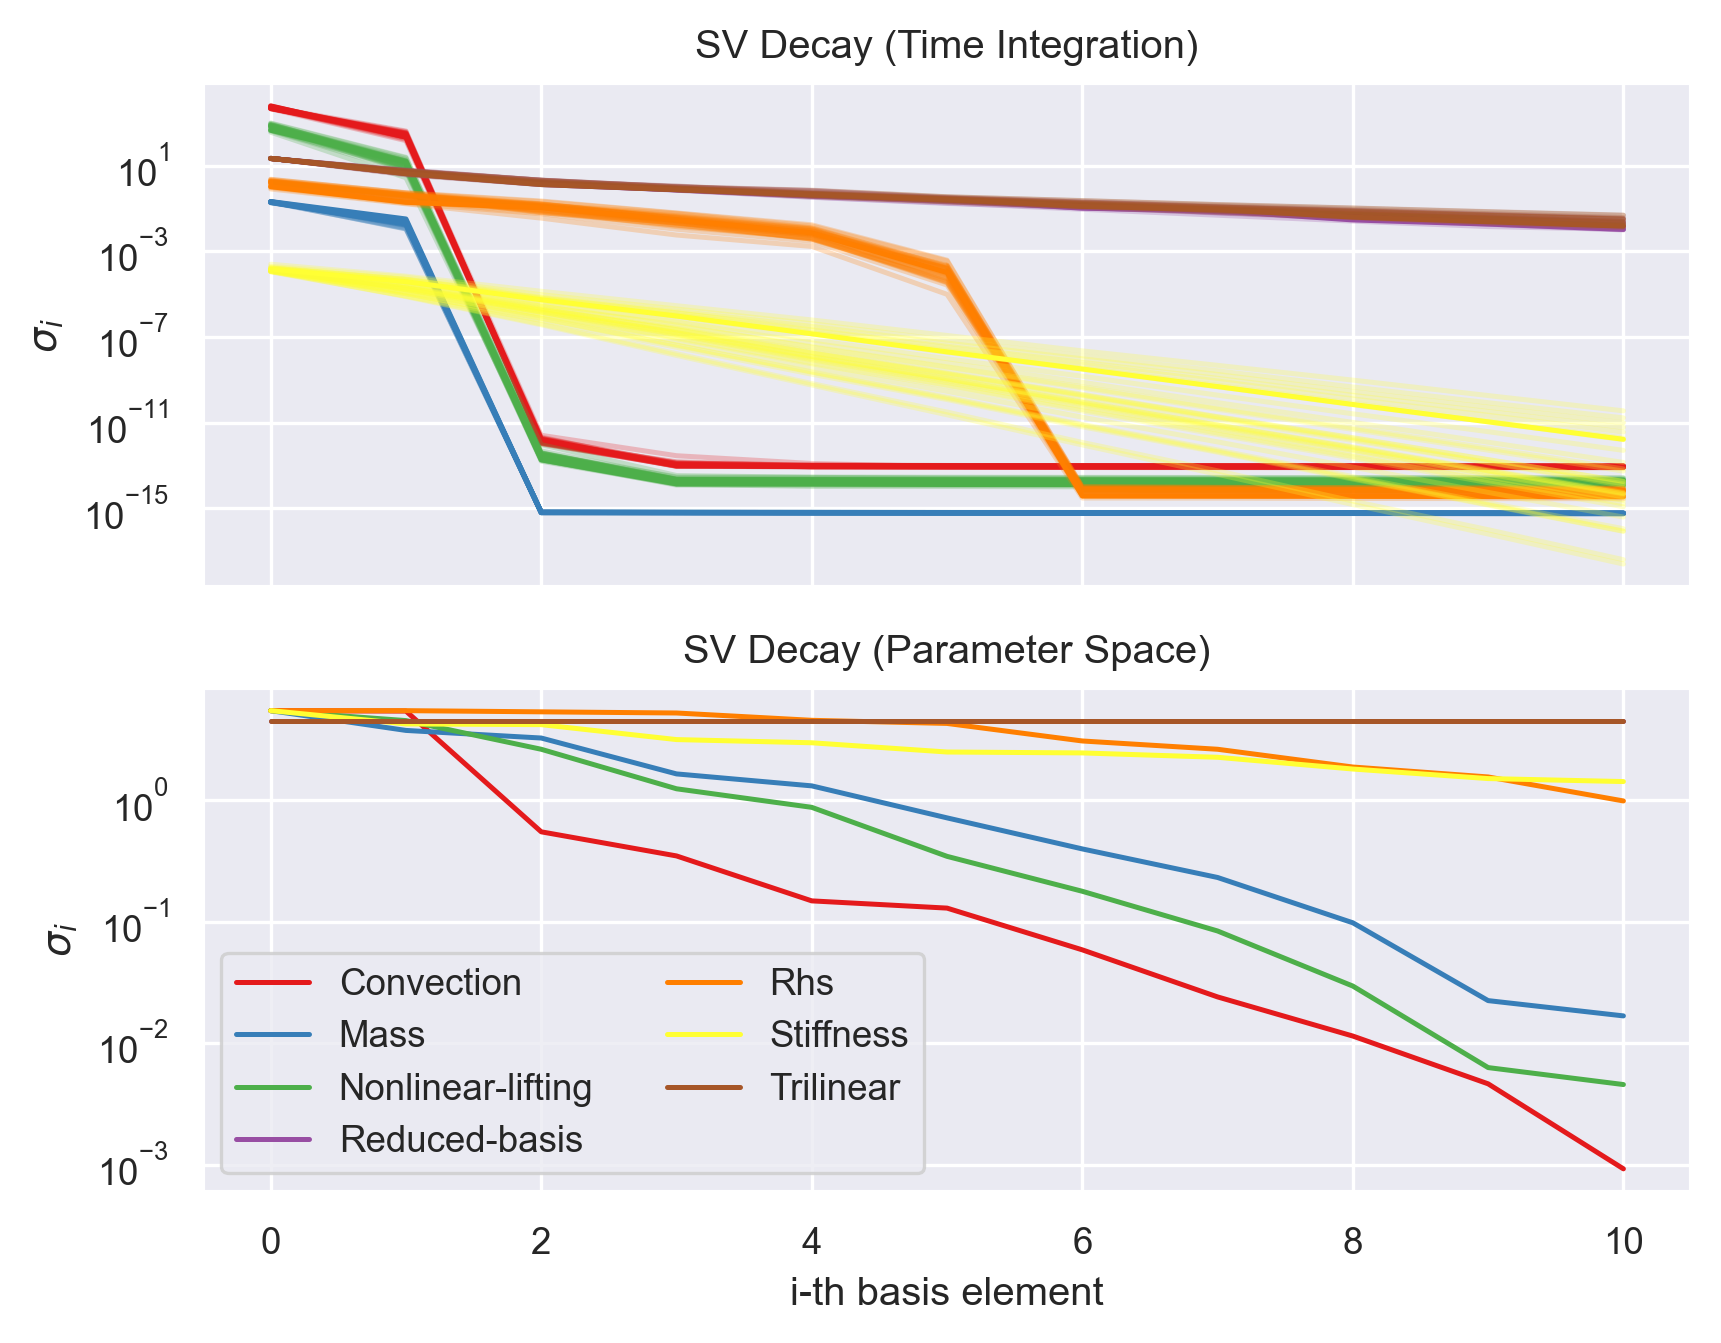
\includegraphics[width =\columnwidth]{research_project/piston/figures/nonlinear_displacement/separable/sigmas_logy.png}
    \caption{This figure is a zoom-in of Figure~\ref{fig:nlinear_disp_sep_loglog}.
    Only the first ten singular values (modes) are shown.
    We can see how for the time integration step most operators 
    are perfectly summarized with two to six modes.
    This is due to the fact that the displacement is separable in time and space;
    and only the space function is nonlinear.}
    \label{fig:nlinear_disp_sep_logy}
\end{figure}

\subsubsection{Operators Error Decay}
Now that we have multiple operators with a non-trivial basis, 
we have to tune simultaneously all of their errors.
To get a glimpse of what that might look like, 
we plot in Figure~\ref{fig:nlinear_disp_operators_error_decay}
the error decay for each operator as a function of the basis percentile size.
The offline and online sampling pools are shown in 
Figure~\ref{fig:nlinear_disp_operators_sampling_space}.

All the errors decay as the basis size increases, 
but each operator needs a different basis size to reach the same error threshold.
For the offline samples, as the basis size is shrunk, 
the errors remain concentrated for different parametrizations.
For the online samples, this behaviour is not present, 
with more dispersion between the different parametrizations.
The errors with the full basis are smaller for the offline pool, 
compared to those from the online pool.
This is an expected behaviour, 
since the basis is optimized for the offline sample.
The trilinear operator errors are very similar for all parametrizations.

\begin{figure}[h]
    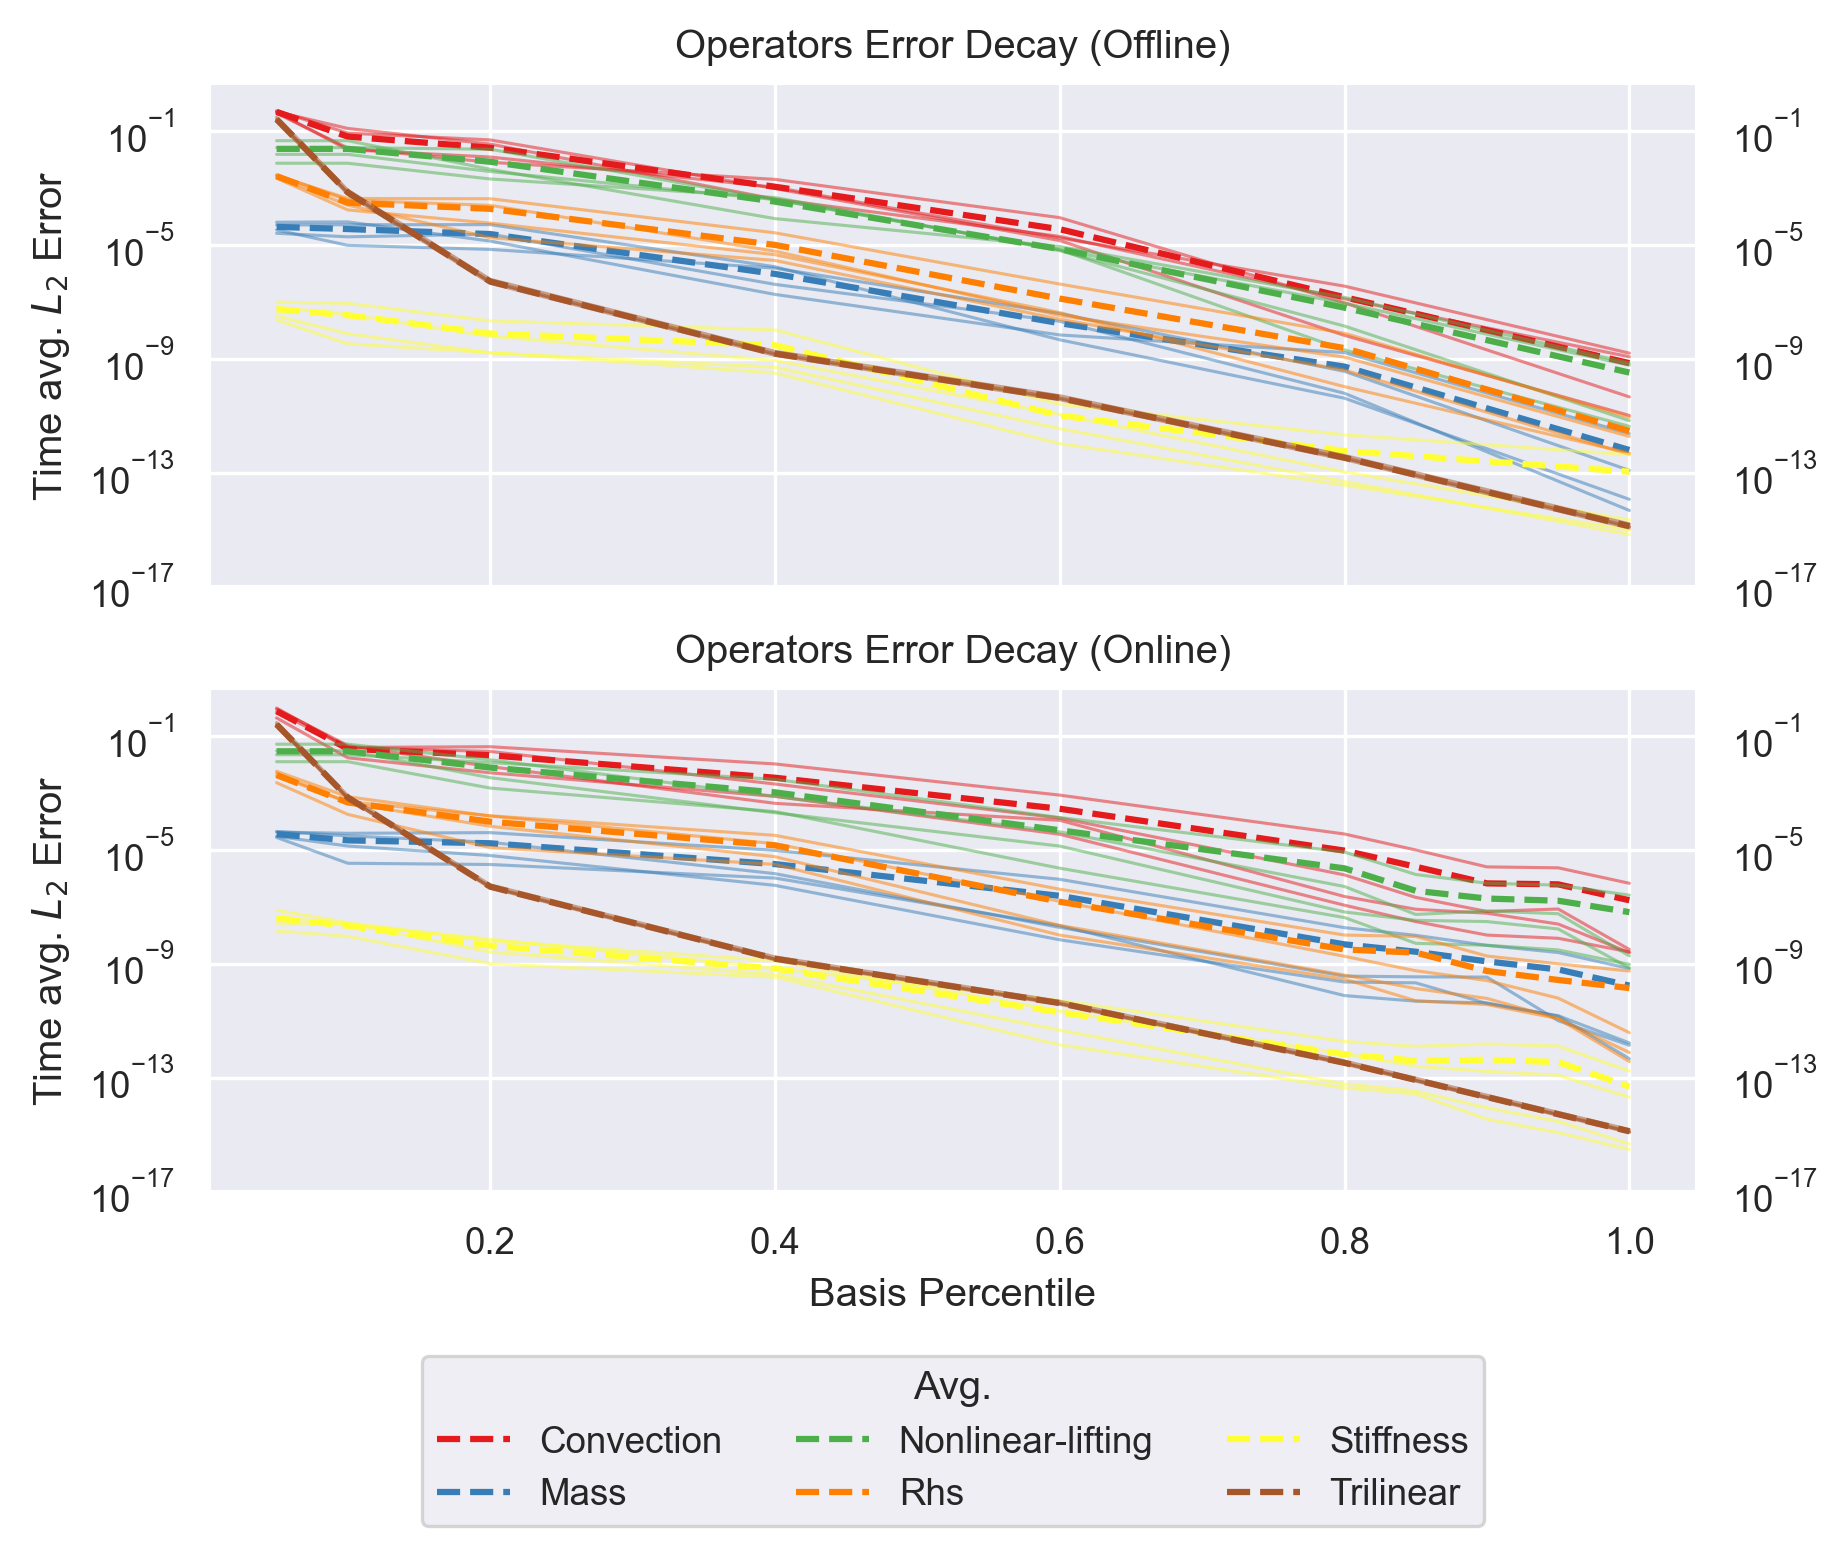
\includegraphics[width =\columnwidth]{research_project/piston/figures/nonlinear_displacement/separable/operators_error_decay_percentile.png}
    \caption{Operator error decay as a function of basis size percentile.
    (Top) Offline parameter sample.
    (Bottom) Online parameter sample.
    All the errors decay as the basis size increases, 
    but each operator needs a different basis size to reach the same error threshold.
    For the offline samples, the errors are concentrated.
    For the online samples, the errors present more dispersion.
    The errors with the full basis are smaller for the offline pool, 
    compared to those from the online pool.
    This is an expected behaviour, 
    since the basis is optimized for the offline sample.
    The trilinear operator errors are very similar for all parametrizations.}
    \label{fig:nlinear_disp_operators_error_decay}
\end{figure}

\clearpage
\subsection{Certification by Truncation: Limits}
We already saw in the heatmap from Figure~\ref{fig:nonlinear_error_decay_heatmap}
in Section~\ref{sec:reduced_basis_mdeim_error_interaction}
how the RB and MDEIM approximation errors could 
set a lower bound to the HROM error.
Now, we are going to further show how this interaction can make 
the HROM certification-by-truncation fail.

To do so, we set the experiments shown in 
Tables~\ref{tab:certification_experiments_grid} 
and~\ref{tab:certification_experiments_results}.
The idea is to see what happens with the error estimator when 
the RB approximation error is below or above the (M)DEIM error.

The conclusion of the experiments is that when the RB error is below the (M)DEIM error,
the HROM error is saturated by operators error;
and hence the model truncation technique cannot be used to certify the HROM results.
When the RB error is above the (M)DEIM error, the trucation technique 
will produce effective error estimations.

\begin{table}[h]
    \centering
    \caption{Numerical experiments configuration. 
    Pure ROM means no (M)DEIM is used.
    HROM means all reduced and collateral bases are used.}
    \begin{tabular}{ccc}
        \toprule                                                           
        & Pure ROM & HROM \\ 
        \midrule                                                           
        $\varepsilon_{\text{RB}}$ > $\varepsilon_{\text{MDEIM}}$ & Figure~\ref{fig:nlinear_disp_no_deim_errors_above_threshold} & Figure~\ref{fig:nlinear_disp_deim_errors_above_threshold}     \\
        $\varepsilon_{\text{RB}}$ < $\varepsilon_{\text{MDEIM}}$ & Figure~\ref{fig:nlinear_disp_no_deim_errors_below_threshold} & Figure~\ref{fig:nlinear_disp_deim_errors_below_threshold} \\
        \bottomrule
    \end{tabular}    
    \label{tab:certification_experiments_grid}
\end{table}
We choose 
\begin{table}[h]
    \centering
    \caption{Numerical experiments summary.}
    \begin{tabular}{ccccc}
        \toprule
        Experiment                                                   & (M)DEIM    & ROM         & SROM       & Estimator \\
        {}                                                           & {}         & $N$, Error  & $N$, Error & {}         \\
        \midrule
        Figure~\ref{fig:nlinear_disp_no_deim_errors_above_threshold} &  -         &  $15 , 10^{-4}$  & $25 , 10^{-6}$ & Accurate  \\
        Figure~\ref{fig:nlinear_disp_no_deim_errors_below_threshold} &  -         &  $25 , 10^{-6}$  & $30 , 10^{-7}$ & Accurate  \\
        Figure~\ref{fig:nlinear_disp_deim_errors_above_threshold}    &  $10^{-6}$ &  $15 , 10^{-3}$  & $25 , 10^{-4}$ & Accurate  \\
        Figure~\ref{fig:nlinear_disp_deim_errors_below_threshold}    &  $10^{-6}$ &  $25 , 10^{-4}$  & $30 , 10^{-4}$ & Ineffective \\
        \bottomrule
    \end{tabular}
    \label{tab:certification_experiments_results}
\end{table}

%tab:arbitrary_displacement_errors_online
%tab:arbitrary_displacement_size_percentile

\begin{figure}[h]
    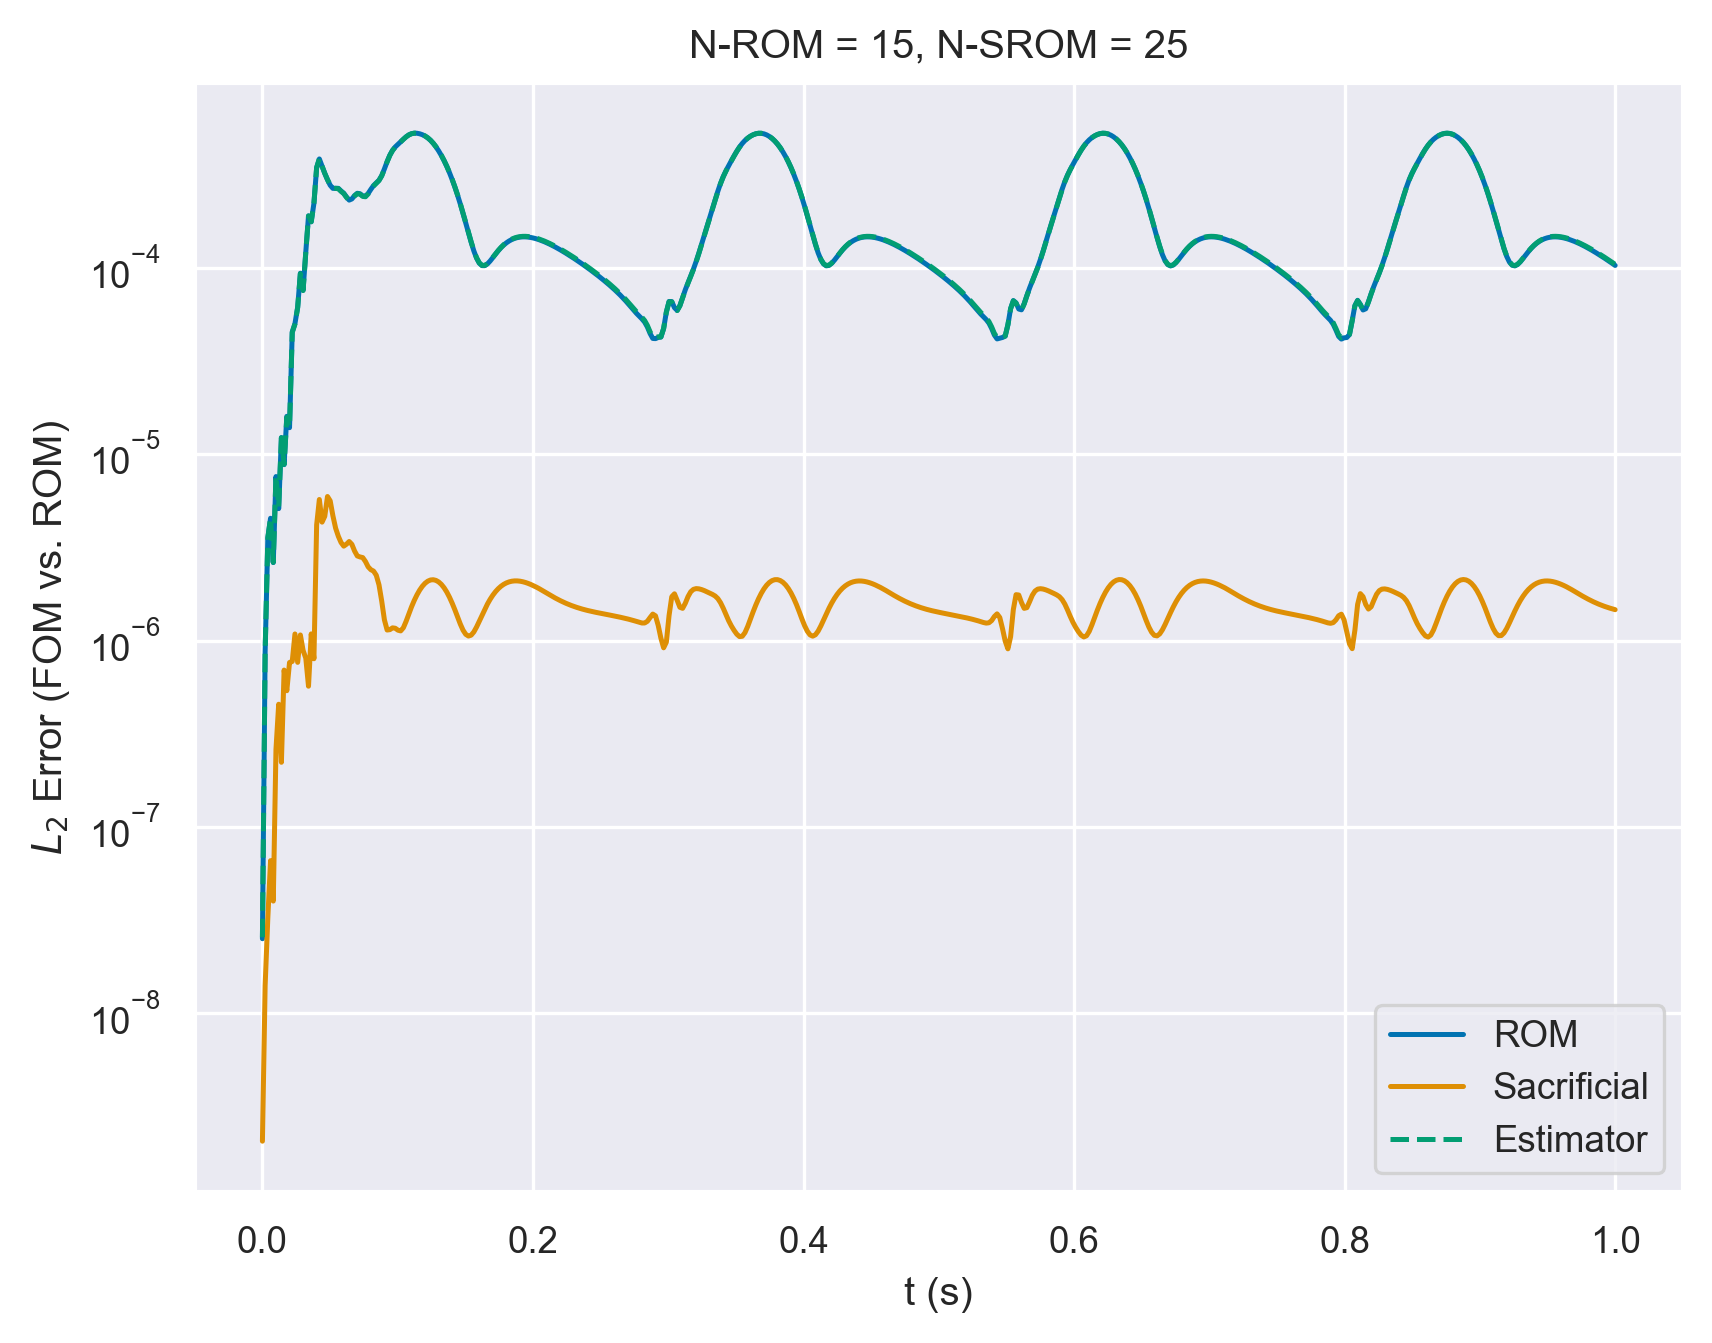
\includegraphics[width =\columnwidth]{research_project/piston/figures/nonlinear_displacement/truncation_error/no_deim/error_estimation_rom_15_srom_25_0.png}
    \caption{ROM vs. FOM approximation error, no (M)DEIM.
    The FOM operators are assembled and projected for each time step.
    The certification-by-truncation procedure is accurate, with the estimator matching the ROM error.}
    \label{fig:nlinear_disp_no_deim_errors_above_threshold}
\end{figure}

\begin{figure}[h]
    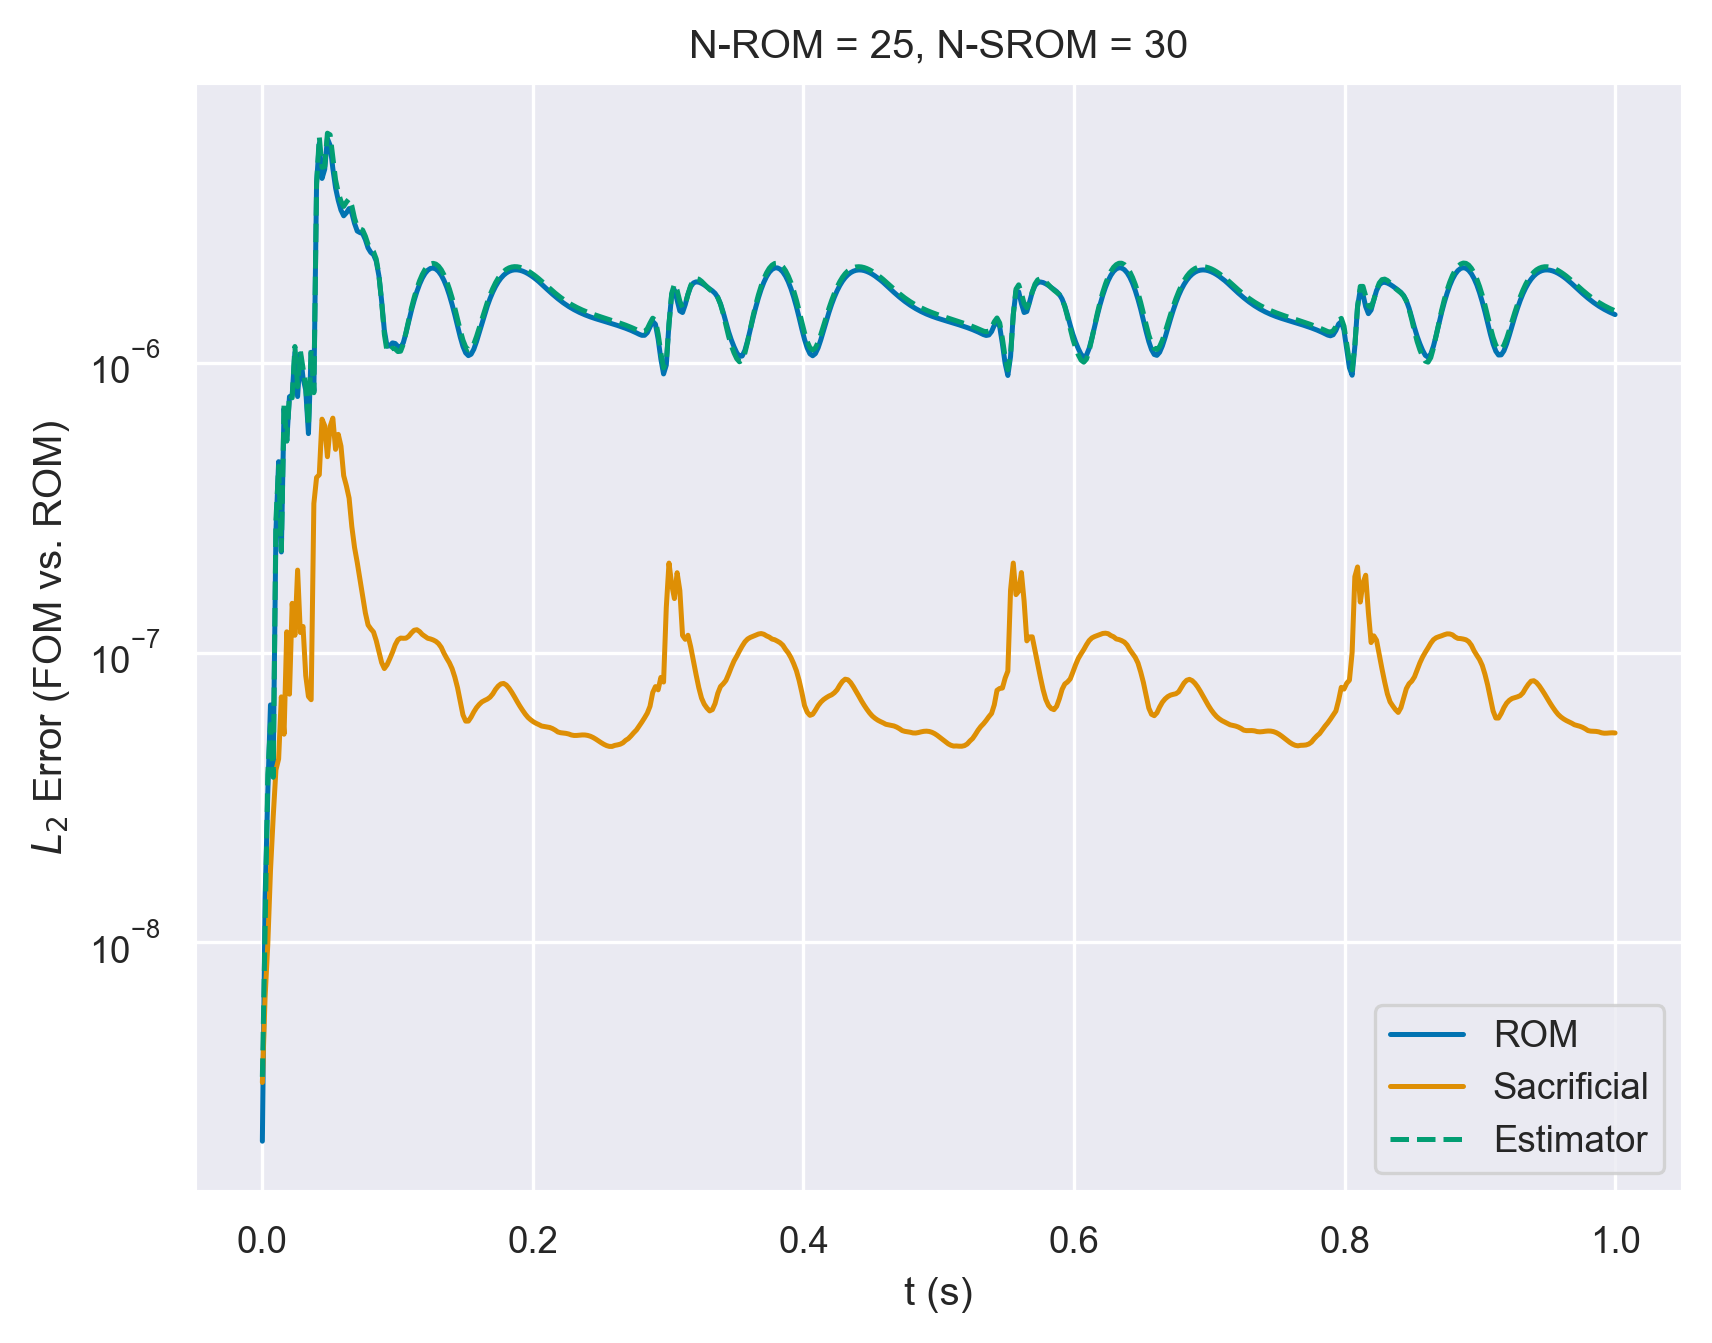
\includegraphics[width =\columnwidth]{research_project/piston/figures/nonlinear_displacement/truncation_error/no_deim/error_estimation_rom_25_srom_30_0.png}
    \caption{ROM vs. FOM approximation error, no (M)DEIM.
    The FOM operators are assembled and projected for each time step.
    The certification-by-truncation procedure is accurate, with the estimator matching the ROM error.}
    \label{fig:nlinear_disp_no_deim_errors_below_threshold}
\end{figure}

\begin{figure}[h]
    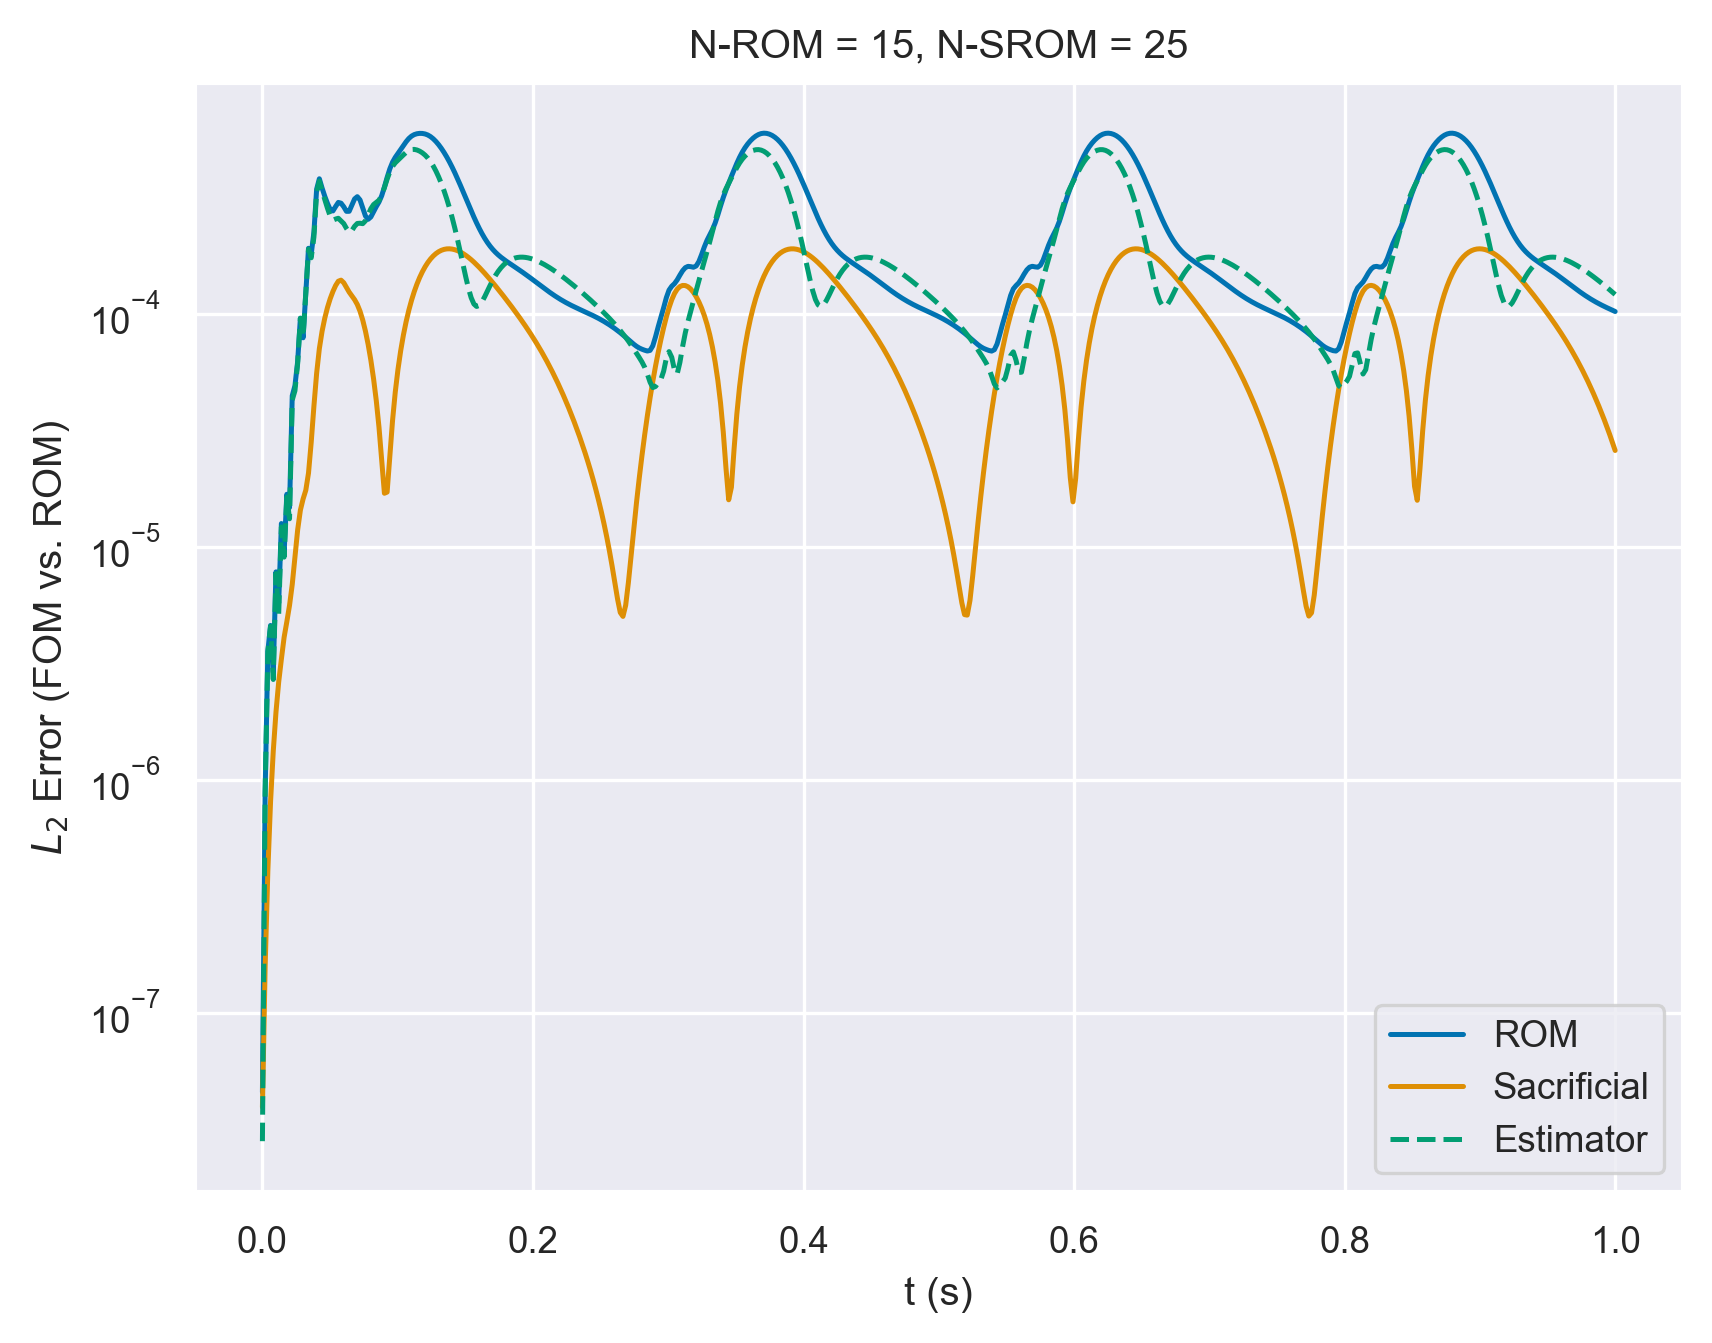
\includegraphics[width =\columnwidth]{research_project/piston/figures/nonlinear_displacement/truncation_error/deim/error_estimation_rom_15_srom_25_0.png}
    \caption{ROM vs. FOM approximation error, (M)DEIM is active.
    The approximation error for all operators is $10^{-6}$.
    The error of the SROM has increased, making it closer to the ROM.
    But since it remains below it, 
    the certification-by-truncation procedure is still perfectly.}
    \label{fig:nlinear_disp_deim_errors_above_threshold}
\end{figure}


\begin{figure}[h]
    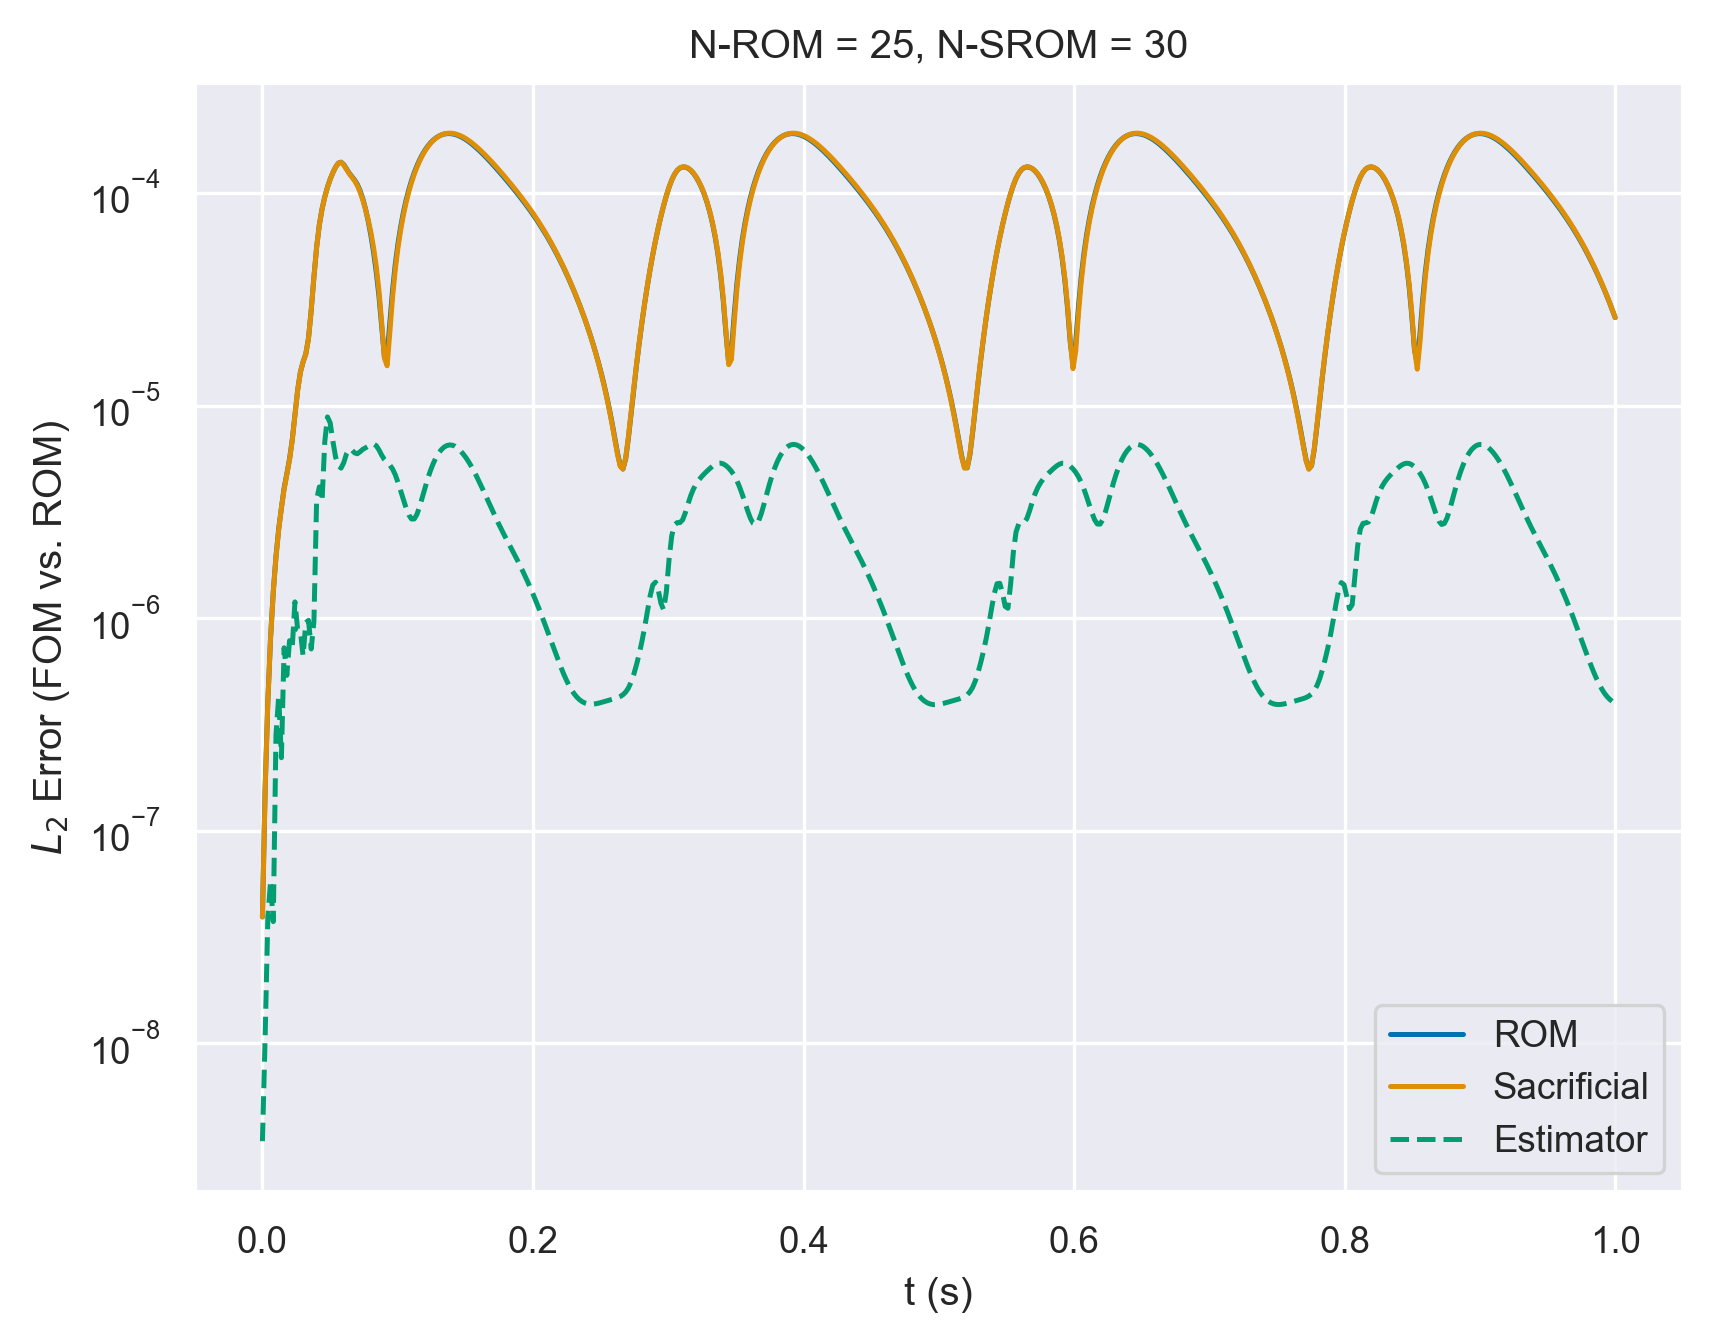
\includegraphics[width =\columnwidth]{research_project/piston/figures/nonlinear_displacement/truncation_error/deim/error_estimation_rom_25_srom_30_0.png}
    \caption{ROM vs. FOM approximation error, (M)DEIM is active.
    The approximation error for all operators is $10^{-6}$.
    The error for the ROM and the SROM is the same, leading to an ineffective truncation estimator.}
    \label{fig:nlinear_disp_deim_errors_below_threshold}
\end{figure}

\clearpage
\subsection{N-MDEIM Basis by Mode Evaluation}
In this final section we build the N-MDEIM basis for the trilinear term
from snapshots obtained from mode evaluations 
(as opposed to snapshots collected during FOM simulation).

We anticipate that we are going to find the same results as the ones that we obtained in
Section~\ref{sec:nmdeim_one_mode}, despite the arbitrary shape of the mesh.
This is due to the following facts:
\begin{itemize}
    \item The domain is one-dimensional.
    \item The FEM basis functions are $\mathbb{P}1$.
    \item The trilinear integrand is linear in all of its arguments, including the parameters.
    \item The trilinear integrand contains the derivative of the trial function $u$.
\end{itemize}
The last fact is crucial. 
Due to this fact, the non-uniform mesh size goes unnoticed, 
since the derivative of the Lagrangian function gets cancelled by the integration.
This only happens in the specific context described in the list above.

Therefore, the 







\end{document}